% Provenance (never printed): see sources/outline_sources.md (Year 2: field and laboratory methods ---
% igneous and metamorphic petrography, chemical analysis by XRF, ICP-MS and microprobe, isotope mass
% spectrometry, a mapping campaign). Modelled on Book 3 ch. 6.
% Textures: BGS RR 99-02 (Robertson 1999), Open University Virtual Microscope, Carleton BH250,
% UCSB Geology 102C (Hacker); QAPF: BGS RR 99-06 (Gillespie and Styles 1999); instruments: SERC
% Geochemical Instrumentation and Analysis sheets (EPMA, WDS, XRF, TIMS, MC-ICPMS); XRF procedure
% and reference-material results: USGS OFR 02-223 and its chapter T (Taggart and Siems 2002); Sr
% isotopes: CIAAW; spike and mass bias: Cheong, Jeong and Kwon (2014). Ledger rows in
% sources/ledger/book4.md; curves and stations from figdata/bachelor-2/labmethods.py, numbers from
% the Book 4 second-writer scratch calculator calc/ch31.py. Observation only: the professional work
% is described in the third person.
\chapter{Métodos de campo y de laboratorio II}\label{ch:b2:field-lab-methods-2}

Cada número de los capítulos de petrología de este libro empezó siendo una roca en una bolsa, una lámina delgada bajo un
microscopio y un polvo en un instrumento. Una composición mineral representada en un diagrama de fases, el
contenido en sílice que da nombre a una lava, la razón isotópica del estroncio que rastrea una fuente del manto: cada uno
salió de una cadena de operaciones que empezó en un afloramiento, y cada uno arrastra los errores de cada
eslabón. Este capítulo sigue esa cadena para las rocas del basamento de las colinas de Varden: la lectura de las texturas
en lámina delgada, el recuento de minerales, el análisis de la roca total, después el de minerales aislados, después el de los isótopos,
preguntándose en cada paso qué calidad tiene el número.

\begin{recall}
\textbf{Del volumen de primer año}: estación de campo, cuaderno de campo, muestra orientada, lámina delgada,
microscopio de polarización, luz polarizada plana, nicoles cruzados; identificación óptica de los minerales
formadores de roca; recálculo de una fórmula mineral a partir de un análisis de óxidos sobre un número fijo de oxígenos,
y del hierro férrico por balance de cargas; foliación y esquistosidad; isócrona, razón inicial y la
recta de mínimos cuadrados. \textbf{De los libros de química}: espectrometría de masas, plasma acoplado inductivamente;
curva de calibración, límite de detección, límite de cuantificación, precisión, veracidad, sesgo,
repetibilidad, desviación típica de la media. \textbf{De los libros de física}: los rayos X característicos
y la ley de Moseley; la ley de Bragg; la tensión superficial; la propagación de incertidumbres.
\textbf{De los libros de matemáticas}: la distribución binomial, su media y su varianza.
\textbf{Del \cref{ch:b2:magmatic-series}}: \omterm{def:b2:magmatic-series:qapf}{composición modal}, \omterm{def:b2:magmatic-series:qapf}{diagrama QAPF}.
\textbf{Del \cref{ch:b2:isotope-geochemistry}}: \omterm{def:b2:isotope-geochemistry:tracer}{trazador isotópico radiogénico}, \omterm{def:b2:isotope-geochemistry:standards}{patrón isotópico de referencia}.
\end{recall}

\section{Petrografía: las texturas como historia}\label{sec:b2:field-lab-methods-2:petrography}

El volumen de primer año usó el microscopio de polarización para identificar minerales. Un petrógrafo lee también
cómo están dispuestos los granos, porque esa disposición registra el orden en que crecieron. Dos
texturas son los testigos más comunes de la cristalización a partir de un fundido y de la recristalización en
estado sólido.

\begin{definition}[Textura ofítica, textura granoblástica]\label{def:b2:field-lab-methods-2:textures}
Una roca ígnea tiene \emph{textura ofítica}\index{textura ofitica@textura ofítica} cuando grandes cristales de piroxeno
engloban pequeños listones de plagioclasa orientados al azar; la textura es típica de la dolerita, el gabro
y el basalto. Una roca metamórfica tiene \emph{textura granoblástica}\index{textura granoblastica@textura granoblástica} cuando
es un agregado de cristales de forma aproximadamente equidimensional y de tamaño parecido, en muchos casos anhedrales,
cuyos límites rectos se encuentran de tres en tres con ángulos cercanos a \ang{120}.
\end{definition}
% ledger: carletonB:ophitic, ouVM:textures, bgsM:textures

En una roca ofítica, los listones englobados están enteros y son euhedrales, y el piroxeno rellena el espacio
entre ellos: la plagioclasa creció primero, y el piroxeno a su alrededor. Los ángulos de \ang{120} de una
\omterm{def:b2:field-lab-methods-2:textures}{textura granoblástica} son los de granos que han tenido tiempo de ajustar sus límites; el material didáctico de petrografía interpreta esas uniones
triples como un signo de equilibrio químico y textural. El ángulo se deduce de un equilibrio de fuerzas: los límites de grano tiran de su
línea común como películas de jabón (la tensión superficial, de los libros de física).
% ledger: ouVM:equilibrium

\begin{proposition}[Ángulos en una unión triple]\label{prop:b2:field-lab-methods-2:triple}
Sean tres límites de grano que se encuentran a lo largo de una línea, con tensiones (energías por unidad de superficie) $\gamma_1$,
$\gamma_2$, $\gamma_3$, y sea $\theta_i$ el ángulo entre los dos límites distintos del
límite $i$. En el equilibrio,
\begin{equation}
\frac{\gamma_1}{\sin\theta_1} = \frac{\gamma_2}{\sin\theta_2} = \frac{\gamma_3}{\sin\theta_3},
\label{eq:b2:field-lab-methods-2:lami}
\end{equation}
y tres tensiones iguales se encuentran formando tres ángulos de \ang{120}.
\end{proposition}

\begin{proof}
En un plano perpendicular a la unión, cada límite tira de la unión a lo largo de su propia traza
con la fuerza $\gamma_i$ por unidad de longitud. En el equilibrio las tres fuerzas suman cero, así que, colocadas
una a continuación de otra, cierran un triángulo. El ángulo del triángulo opuesto al lado $\gamma_i$ es
$\pi - \theta_i$, cuyo seno es $\sin\theta_i$, y el teorema de los senos en el triángulo da
\eqref{eq:b2:field-lab-methods-2:lami}. Si las tres tensiones son iguales, el triángulo es
equilátero y cada ángulo exterior $\theta_i$ vale $\pi - \pi/3 = 2\pi/3$, es decir, \ang{120}.
\end{proof}

\begin{omfigure}
\centering
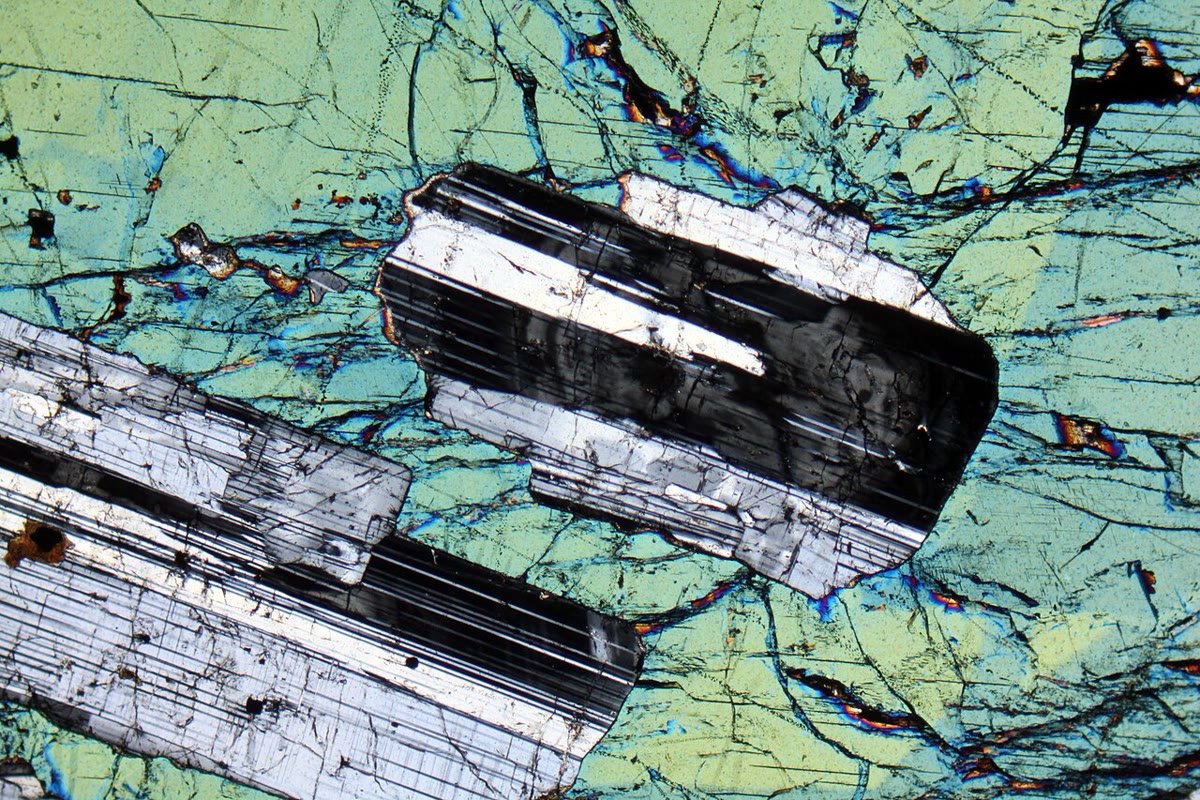
\includegraphics[height=4.6cm]{images/book4/b2-31-ophitic.jpg}\quad
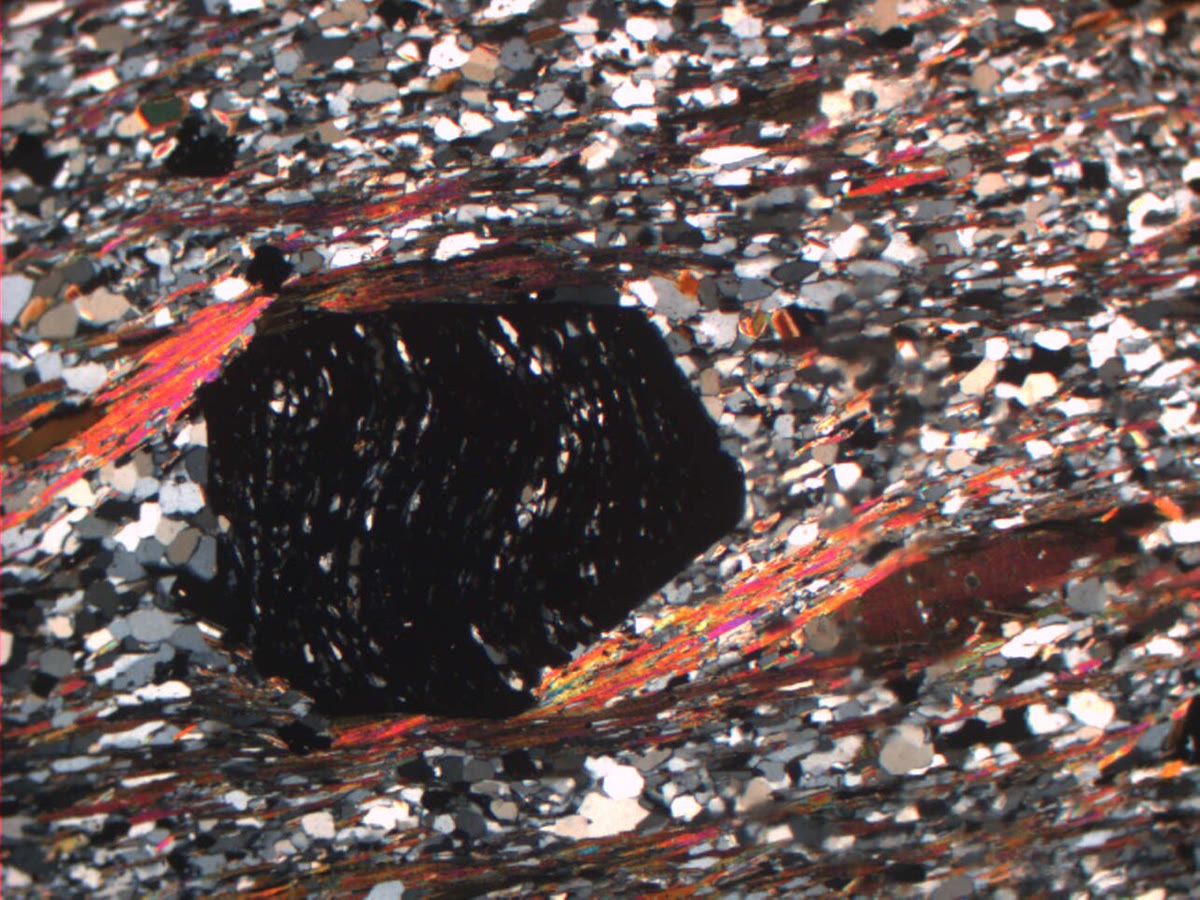
\includegraphics[height=4.6cm]{images/book4/b2-31-garnet-porphyroblast.jpg}
\par\smallskip{\small Dos texturas con nicoles cruzados. Izquierda: un solo cristal de augita (azul
y verde) engloba listones de plagioclasa rayados por sus maclas, la disposición de una \omterm{def:b2:field-lab-methods-2:textures}{textura
ofítica}; campo de visión de \qty{7}{mm}. Fotografía Strekeisen, CC BY-SA 4.0 (Wikimedia Commons).
Derecha: un esquisto de granate y mica. El granate, negro porque es isótropo, es un gran cristal que
creció en estado sólido; inclusiones de cuarzo lo atraviesan en trenes, y la foliación de moscovita
(colores vivos), biotita (marrón) y cuarzo (gris) se curva a su alrededor. Fotografía Jackdann88,
CC BY 3.0 (Wikimedia Commons).}
\end{omfigure}
% ledger: photo:b2-31-ophitic, photo:b2-31-garnet

Los minerales metamórficos no crecen todos al mismo ritmo. Algunas especies crecen sobre las demás hasta formar cristales muy grandes,
que engloban los granos pequeños que los rodean a medida que crecen.

\begin{definition}[Porfiroblasto, poiquiloblasto, tren de inclusiones, corona]\label{def:b2:field-lab-methods-2:porphyroblast}
Un \emph{porfiroblasto}\index{porfiroblasto} es un cristal grande que creció durante el \omterm{def:b2:metamorphic-facies:metamorphism}{metamorfismo}
dentro de una matriz de grano más fino; los forman el granate, la estaurolita, la cordierita y el cloritoide, de
milímetros a varios centímetros de diámetro. Un \emph{poiquiloblasto}\index{poiquiloblasto} es un
porfiroblasto que contiene muchas inclusiones de otros minerales. Un \emph{tren de
inclusiones}\index{tren de inclusiones} es una línea de inclusiones alineadas dentro de un porfiroblasto, que
conserva la fábrica de la matriz en el momento en que el cristal creció sobre ella. Una
\emph{corona}\index{corona (textura de reacción)} es un borde de uno o varios minerales nuevos que rodea por completo
a un mineral que se estaba descomponiendo porque había dejado de ser estable con sus
vecinos: una textura de reacción, congelada antes de que la reacción se completara.
\end{definition}
% ledger: bgsM:textures, ouVM:textures

Comparar el \omterm{def:b2:field-lab-methods-2:porphyroblast}{tren de inclusiones} ($S_i$, la fábrica interna) con la foliación exterior al cristal
($S_e$, la fábrica externa) data el crecimiento de un \omterm{def:b2:field-lab-methods-2:porphyroblast}{porfiroblasto} respecto de la deformación que
produjo la foliación. Los criterios siguientes, dibujados en la figura, son los de los apuntes didácticos habituales.
% ledger: ucsbH:inclusion-trails

\begin{method}[Datación relativa de un porfiroblasto por sus trenes de inclusiones]\label{met:b2:field-lab-methods-2:timing}
Búsquese una sección cortada perpendicularmente a la foliación y compárense $S_i$ y $S_e$.
\begin{enumerate}
  \item \textbf{Inclusiones al azar}, $S_e$ desviada alrededor del cristal: creció antes de que se
        formara la foliación (\emph{pretectónico}).
  \item \textbf{$S_i$ rectilínea cortada en el borde}, discontinua con una $S_e$ desviada: creció
        sobre una foliación anterior, entre dos deformaciones (\emph{intertectónico}).
  \item \textbf{$S_i$ curvada}, continua con $S_e$: creció mientras se formaba la foliación, girando
        o siendo englobado mientras crecía (\emph{sintectónico}; la espiral de un granate en bola de nieve).
  \item \textbf{$S_i$ rectilínea continua con una $S_e$ no desviada}: creció después de la foliación
        (\emph{postectónico}).
\end{enumerate}
\end{method}

\begin{omfigure}
\centering
\begin{tikzpicture}[x=1cm, y=1cm, font=\scriptsize]
% schematic after the criteria of ledger ucsbH:inclusion-trails
% panel 1: pre-tectonic
\begin{scope}[shift={(0,0)}]
\draw[omExo, line width=0.5pt] (-1.5,0.95) .. controls (-0.6,0.95) and (-0.5,0.85) .. (0,0.85) .. controls (0.5,0.85) and (0.6,0.95) .. (1.5,0.95);
\draw[omExo, line width=0.5pt] (-1.5,-0.95) .. controls (-0.6,-0.95) and (-0.5,-0.85) .. (0,-0.85) .. controls (0.5,-0.85) and (0.6,-0.95) .. (1.5,-0.95);
\draw[omExo, line width=0.5pt] (-1.5,0.45) .. controls (-0.9,0.45) and (-0.85,0.78) .. (0,0.78) .. controls (0.85,0.78) and (0.9,0.45) .. (1.5,0.45);
\draw[omExo, line width=0.5pt] (-1.5,-0.45) .. controls (-0.9,-0.45) and (-0.85,-0.78) .. (0,-0.78) .. controls (0.85,-0.78) and (0.9,-0.45) .. (1.5,-0.45);
\draw[omExo, line width=0.5pt] (-1.5,0) -- (-0.78,0); \draw[omExo, line width=0.5pt] (0.78,0) -- (1.5,0);
\filldraw[fill=omThm!15, draw=omThm, line width=0.6pt] (0,0) circle (0.72);
\draw[black, line width=0.7pt] (-0.4,0.2) -- (-0.25,0.35); \draw[black, line width=0.7pt] (0.1,0.35) -- (0.3,0.2);
\draw[black, line width=0.7pt] (-0.35,-0.2) -- (-0.15,-0.25); \draw[black, line width=0.7pt] (0.2,-0.15) -- (0.25,-0.4);
\draw[black, line width=0.7pt] (-0.05,0.05) -- (0.05,-0.1); \draw[black, line width=0.7pt] (0.35,0.0) -- (0.5,0.12);
\node at (0,-1.3) {pretectónico};
\end{scope}
% panel 2: inter-tectonic
\begin{scope}[shift={(3.4,0)}]
\draw[omExo, line width=0.5pt] (-1.5,0.95) .. controls (-0.6,0.95) and (-0.5,0.85) .. (0,0.85) .. controls (0.5,0.85) and (0.6,0.95) .. (1.5,0.95);
\draw[omExo, line width=0.5pt] (-1.5,-0.95) .. controls (-0.6,-0.95) and (-0.5,-0.85) .. (0,-0.85) .. controls (0.5,-0.85) and (0.6,-0.95) .. (1.5,-0.95);
\draw[omExo, line width=0.5pt] (-1.5,0.45) .. controls (-0.9,0.45) and (-0.85,0.78) .. (0,0.78) .. controls (0.85,0.78) and (0.9,0.45) .. (1.5,0.45);
\draw[omExo, line width=0.5pt] (-1.5,-0.45) .. controls (-0.9,-0.45) and (-0.85,-0.78) .. (0,-0.78) .. controls (0.85,-0.78) and (0.9,-0.45) .. (1.5,-0.45);
\draw[omExo, line width=0.5pt] (-1.5,0) -- (-0.78,0); \draw[omExo, line width=0.5pt] (0.78,0) -- (1.5,0);
\filldraw[fill=omThm!15, draw=omThm, line width=0.6pt] (0,0) circle (0.72);
\begin{scope}
\clip (0,0) circle (0.66);
\foreach \k in {-0.6,-0.3,0,0.3,0.6} {\draw[black, line width=0.7pt, dash pattern=on 2pt off 1.5pt] (-0.8,\k-0.45) -- (0.8,\k+0.45);}
\end{scope}
\node at (0,-1.3) {intertectónico};
\end{scope}
% panel 3: syn-tectonic
\begin{scope}[shift={(6.8,0)}]
\draw[omExo, line width=0.5pt] (-1.5,0.8) -- (1.5,0.8);
\draw[omExo, line width=0.5pt] (-1.5,-0.8) -- (1.5,-0.8);
\draw[omExo, line width=0.5pt] (-1.5,0.4) -- (-0.6,0.4); \draw[omExo, line width=0.5pt] (0.6,0.4) -- (1.5,0.4);
\draw[omExo, line width=0.5pt] (-1.5,0) -- (-0.72,0); \draw[omExo, line width=0.5pt] (0.72,0) -- (1.5,0);
\draw[omExo, line width=0.5pt] (-1.5,-0.4) -- (-0.6,-0.4); \draw[omExo, line width=0.5pt] (0.6,-0.4) -- (1.5,-0.4);
\filldraw[fill=omThm!15, draw=omThm, line width=0.6pt] (0,0) circle (0.72);
\draw[black, line width=0.7pt, dash pattern=on 2pt off 1.5pt] (-0.6,0.4) .. controls (-0.35,0.4) and (-0.2,0.3) .. (-0.05,0.4) .. controls (0.1,0.5) and (0.35,0.4) .. (0.6,0.4);
\draw[black, line width=0.7pt, dash pattern=on 2pt off 1.5pt] (-0.72,0) .. controls (-0.3,0) and (-0.3,-0.45) .. (0,0) .. controls (0.3,0.45) and (0.3,0) .. (0.72,0);
\draw[black, line width=0.7pt, dash pattern=on 2pt off 1.5pt] (-0.6,-0.4) .. controls (-0.35,-0.4) and (-0.1,-0.5) .. (0.05,-0.4) .. controls (0.2,-0.3) and (0.35,-0.4) .. (0.6,-0.4);
\node at (0,-1.3) {sintectónico};
\end{scope}
% panel 4: post-tectonic
\begin{scope}[shift={(10.2,0)}]
\foreach \k in {-0.8,-0.4,0,0.4,0.8} {\draw[omExo, line width=0.5pt] (-1.5,\k) -- (1.5,\k);}
\filldraw[fill=omThm!15, draw=omThm, line width=0.6pt] (0,0) circle (0.72);
\begin{scope}
\clip (0,0) circle (0.66);
\foreach \k in {-0.8,-0.4,0,0.4,0.8} {\draw[black, line width=0.7pt, dash pattern=on 2pt off 1.5pt] (-0.8,\k) -- (0.8,\k);}
\end{scope}
\node at (0,-1.3) {postectónico};
\end{scope}
\end{tikzpicture}
\par\smallskip{\small \omterm{def:b2:field-lab-methods-2:porphyroblast}{Trenes de inclusiones} (negro, discontinuo) en un \omterm{def:b2:field-lab-methods-2:porphyroblast}{porfiroblasto} (rojo) y la foliación
exterior a él (gris), en secciones perpendiculares a la foliación (esquema). De izquierda a derecha:
inclusiones crecidas antes de la foliación, que se curva alrededor del cristal; una fábrica anterior rectilínea cortada
en el borde; un tren que se curva hasta enlazar con la foliación, porque el cristal giró mientras crecía; un
tren rectilíneo que prolonga la foliación no perturbada.}
\end{omfigure}

La petrografía también es cuantitativa. Las proporciones de los minerales de una roca ígnea de grano grueso
le dan nombre en el \omterm{def:b2:magmatic-series:qapf}{diagrama QAPF} (\cref{ch:b2:magmatic-series}), y se miden al
microscopio.

\begin{definition}[Análisis modal, recuento de puntos]\label{def:b2:field-lab-methods-2:modal}
Un \emph{análisis modal}\index{analisis modal@análisis modal} es la medida de la \omterm{def:b2:magmatic-series:qapf}{composición modal} de una
roca. En el \emph{recuento de puntos}\index{recuento de puntos}, una lámina
delgada se desplaza bajo la cruz filar del microscopio en pasos iguales a lo largo de una malla regular, y
en cada punto se anota el mineral que queda bajo la cruz filar; la proporción de puntos que
caen sobre un mineral estima su proporción en la roca.
\end{definition}

\begin{proposition}[Qué mide el recuento de puntos, y con qué calidad]\label{prop:b2:field-lab-methods-2:counting}
(a) En una roca sin orientación preferente, la fracción de área de un mineral en una sección colocada
al azar tiene, en promedio, el valor de su fracción de volumen. (b) Si $n$ puntos caen de forma independiente
sobre un mineral de fracción de área $p$, la proporción contada $\hat p = k/n$ tiene media $p$ y desviación
típica
\begin{equation}
\sigma = \sqrt{\frac{p(1-p)}{n}} , \qquad\text{de modo que se necesitan}\qquad n = \frac{p(1-p)}{\sigma^2}
\label{eq:b2:field-lab-methods-2:binomial}
\end{equation}
puntos para alcanzar una desviación típica $\sigma$.
\end{proposition}

\begin{proof}
(a) Córtese un bloque de roca de altura $H$ en secciones paralelas de área $S$. El volumen del
mineral es $\int_0^H a(z)\,\mathrm{d}z$, donde $a(z)$ es su área en la sección a la altura $z$;
dividiendo por el volumen $SH$, la fracción de volumen es la media de la fracción de área $a(z)/S$ sobre
todas las alturas, que es el valor esperado para una altura elegida al azar. (b) Cada punto cae sobre el
mineral con probabilidad $p$, independientemente de los demás, así que el número $k$ de aciertos sigue la
distribución binomial de parámetros $n$ y $p$, de media $np$ y varianza $np(1-p)$. Dividir por
$n$ da la media $p$ y la varianza $p(1-p)/n$ de $\hat p$.
\end{proof}

La demostración de (b) supone puntos independientes, a lo que se aproxima un paso de malla mayor que los granos.
Para un mineral que constituye el \qty{30}{\percent} de una roca, 500 puntos dan $\sigma =
\sqrt{0.3 \times 0.7/500} = 0.020$, dos puntos porcentuales; llegar a un punto porcentual requiere
$0.21/0.01^2 = 2100$ puntos, cuatro veces más, porque $\sigma$ solo disminuye como $1/\sqrt n$. El
error relativo, $\sigma/p = \sqrt{(1-p)/(np)}$, es máximo para los minerales escasos (figura de abajo,
izquierda). Las proporciones contadas se recalculan después para dar nombre a la roca: una moda con un
\qty{10}{\percent} de cuarzo, 30 de feldespato alcalino, 20 de plagioclasa y 40 de minerales máficos da Q, A y
P de 16.7, 50.0 y 33.3 una vez llevados los tres componentes félsicos a una suma de 100. En el triángulo
QAP, una roca con Q entre 20 y 60 es un granito cuando su razón P/(A+P) está entre el 10 y el
\qty{65}{\percent}: un sienogranito por debajo de 35, un monzogranito por encima; de 65 a 90 es una
granodiorita, por encima de 90 una tonalita. El índice de color $M'$ es la proporción de minerales oscuros, es
decir, de los minerales máficos y afines distintos de la moscovita, el apatito y el carbonato primario; una roca es
leucocrática por debajo de 35, mesocrática de 35 a 65 y melanocrática de 65 a 90.
% ledger: bgsI:qapf, bgsI:colour-index

\begin{omfigure}
\centering
\begin{minipage}[b]{0.49\linewidth}\centering
\begin{tikzpicture}
\begin{axis}[omrecord, width=0.96\linewidth, height=5.0cm, xmode=log, xmin=100, xmax=3000,
  ymin=0, ymax=45, xlabel={puntos contados, $n$}, ylabel={error relativo $\sigma/p$ (\unit{\percent})},
  xtick={100,300,1000,3000}, xticklabels={100,300,1000,3000}, log ticks with fixed point,
  tick label style={font=\scriptsize}, label style={font=\small}]
% computed in figdata/bachelor-2/labmethods.py part pc (binomial counting)
\addplot[omThm, line width=1.1pt] table[x=n, y=rel05] {figdata/out/bachelor-2-labmethods-pc.dat};
\addplot[omProp, line width=1.1pt] table[x=n, y=rel20] {figdata/out/bachelor-2-labmethods-pc.dat};
\addplot[omDef, line width=1.1pt] table[x=n, y=rel50] {figdata/out/bachelor-2-labmethods-pc.dat};
\node[font=\scriptsize, text=omThm, anchor=south west] at (axis cs:330,24) {$p = 0.05$};
\node[font=\scriptsize, text=omProp, anchor=south west] at (axis cs:104,21.5) {$p = 0.2$};
\node[font=\scriptsize, text=omDef, anchor=south west] at (axis cs:104,10.3) {$p = 0.5$};
\end{axis}
\end{tikzpicture}
\end{minipage}\hfill
\begin{minipage}[b]{0.49\linewidth}\centering
\begin{tikzpicture}
\begin{axis}[omrecord, width=0.96\linewidth, height=5.0cm, xmin=52, xmax=76, ymin=-1.0, ymax=0.75,
  xlabel={\ce{SiO2} recomendado (\unit{\percent})}, ylabel={diferencia (\unit{\percent})},
  tick label style={font=\scriptsize}, label style={font=\small},
  ytick={-0.8,-0.4,0,0.4}, yticklabel style={/pgf/number format/fixed}]
% data: figdata/bachelor-2/labmethods.py part xrf; ledger: usgsT:sio2-table
\addplot[black!40, densely dotted] coordinates {(52,0) (76,0)};
\addplot[only marks, mark=*, mark size=1.5pt, omDef, error bars/.cd, y dir=both, y explicit]
  table[x=rec, y=diff, y error=s] {figdata/out/bachelor-2-labmethods-xrf.dat};
\node[font=\scriptsize, anchor=east] at (axis cs:73.0,-0.62) {RGM-1};
\node[font=\scriptsize, anchor=west] at (axis cs:56.6,0.40) {JA-2};
\node[font=\scriptsize, anchor=west] at (axis cs:60.8,-0.55) {AMH-1};
\node[font=\scriptsize, anchor=north] at (axis cs:54.1,-0.10) {BCR-2};
\end{axis}
\end{tikzpicture}
\end{minipage}
\par\smallskip{\small Izquierda: error típico relativo de una proporción modal $p$ medida por \omterm{def:b2:field-lab-methods-2:modal}{recuento de
puntos}, \eqref{eq:b2:field-lab-methods-2:binomial}, para un mineral escaso, uno común y uno abundante.
Derecha: exactitud de la sílice por fluorescencia de rayos X sobre \omterm{def:b2:field-lab-methods-2:xrf}{perlas fundidas} para diez materiales de referencia de rocas,
del basalto al granito; cada punto es la media de 2 a 30 análisis menos el valor recomendado, con
la desviación típica de los análisis como barra. Datos: Taggart y Siems (2002), USGS.}
\end{omfigure}
% ledger: usgsT:sio2-table

\section{Análisis de roca total}\label{sec:b2:field-lab-methods-2:whole-rock}

Un análisis de roca total necesita una muestra representativa de la roca: una ficha didáctica de la colección de
geoquímica del SERC aconseja recoger una muestra varias veces mayor que el grano más grande,
que se tritura por etapas y se muele hasta obtener un polvo fino. El caballo de batalla para los elementos mayores es la
fluorescencia de rayos X. Un haz de rayos X, por lo general de un tubo con ánodo de rodio, arranca electrones
internos de los átomos de la muestra, y cada elemento emite entonces rayos X a sus propias
energías características (ley de Moseley, de los libros de física).
% ledger: sercX:xrf-scope

\begin{definition}[Análisis por fluorescencia de rayos X, perla fundida, pérdida por calcinación]\label{def:b2:field-lab-methods-2:xrf}
El \emph{análisis por fluorescencia de rayos X}\index{analisis por fluorescencia de rayos X@análisis por fluorescencia de rayos X} mide las concentraciones
de los elementos de un sólido a partir de las intensidades de los rayos X característicos que emite bajo un
haz de rayos X, por comparación con patrones de composición conocida. Una \emph{perla
fundida}\index{perla fundida} es un disco de vidrio obtenido fundiendo un polvo de roca pesado con un fundente pesado,
como el tetraborato de litio, y vertiendo el fundido en un molde; es homogénea fueran cuales fueran los granos del
polvo. La \emph{pérdida por calcinación}\index{perdida por calcinacion@pérdida por calcinación} es la fracción de su masa que
pierde un polvo al calentarlo a una temperatura alta fija, sobre todo agua y dióxido de carbono expulsados.
\end{definition}
% ledger: sercX:xrf-scope, usgsT:procedure

La intensidad de una línea es proporcional a la abundancia de su elemento solo cuando las muestras y
los patrones se parecen, ya que los demás elementos absorben y refuerzan la radiación: estos efectos de
matriz, y los del tamaño de grano, son la razón de que el polvo se funda en un vidrio, y de que se aplique todavía una
corrección matemática. La XRF mide los diez elementos mayores y, por encima de alrededor de \qty{1}{ppm},
elementos traza como Rb, Sr, Zr y Ba, con límites de detección de unas pocas partes por millón. Es
débil para los elementos ligeros (número atómico inferior a 11) y no ve ni los isótopos ni el estado de oxidación
del hierro.
% ledger: sercX:xrf-scope, usgsT:procedure

\begin{inthelab}[Una tanda de perlas fundidas]
En un procedimiento publicado por el US Geological Survey, \qty{0.8000}{g} de polvo de roca se calientan en un
crisol de platino y oro a \qty{925}{\celsius} durante 40 minutos, y la pérdida de masa se registra como
\omterm{def:b2:field-lab-methods-2:xrf}{pérdida por calcinación}. Se añade tetraborato de litio, lo suficiente para que queden \qty{8.0000}{g} tras la fusión;
siete crisoles a la vez se mantienen en un horno a \qty{1120}{\celsius} y se balancean durante 35 minutos,
y después se vierten en moldes. En el espectrómetro, un tubo de rodio de ventana frontal irradia cada perla, y
las intensidades de los diez elementos mayores se comparan con las de los patrones. Un análisis cuyos
óxidos suman menos del 97 o más del \qty{101}{\percent} se repite; un analista completa
unas 250 muestras al mes.
\end{inthelab}
% ledger: usgsT:procedure

Los propios patrones son rocas, analizadas tantas veces que su composición se conoce mejor de lo que
puede medirla cualquier análisis aislado.

\begin{definition}[Material de referencia geoquímico]\label{def:b2:field-lab-methods-2:rm}
Un \emph{material de referencia geoquímico}\index{material de referencia geoquimico@material de referencia geoquímico} es una roca, un
mineral o un sedimento natural, molido y homogeneizado en un lote grande, para el que una o varias concentraciones
tienen valores bien establecidos o certificados, y que se usa para calibrar instrumentos y comprobar la exactitud
de un método.
\end{definition}
% ledger: usgsOFR:rm

El basalto BHVO-2 del USGS, recogido en 1995 en una lava que se desbordó del cráter Halemaumau del
Kilauea en 1919, tiene un \ce{SiO2} recomendado del \qty{49.60}{\percent} y \qty{394.1}{ppm} de
estroncio. Un laboratorio comprueba su propia veracidad analizando esos materiales como muestras desconocidas, en los extremos bajo,
medio y alto de su intervalo: en la figura anterior, el método del USGS recupera la sílice a menos del
\qty{0.6}{\percent} del valor recomendado para las diez rocas, de un \ce{SiO2} del 54 al
\qty{74}{\percent}. Sus blancos fijan sus límites: el límite de detección se toma como tres desviaciones
típicas de blancos preparados de forma independiente, el límite inferior de notificación como cinco, y a menudo se
proponen diez para el límite de cuantificación.
% ledger: usgs:bhvo2-origin, usgs:bhvo2-major, usgs:bhvo2-trace, usgsOFR:rm, usgsOFR:lod, usgsT:sio2-table

\begin{method}[Calibración y control de un análisis de roca total]\label{met:b2:field-lab-methods-2:calibration}
\begin{enumerate}
  \item \textbf{Calibrar.} Mídase la intensidad $I$ de cada elemento en perlas de varios materiales de
        referencia, y ajústese la recta de mínimos cuadrados $c = aI + b$ de la concentración recomendada
        frente a la intensidad.
  \item \textbf{Medir.} Conviértase la intensidad de cada muestra desconocida en una concentración con la recta.
  \item \textbf{Controlar.} Analícese un material de referencia como desconocido en cada tanda y compárese con
        su valor recomendado; súmense los óxidos y la \omterm{def:b2:field-lab-methods-2:xrf}{pérdida por calcinación}, que deberían acercarse
        al \qty{100}{\percent}.
  \item \textbf{Informar.} Dese el análisis tal como se midió, con su \omterm{def:b2:field-lab-methods-2:xrf}{pérdida por calcinación}; para los
        diagramas de clasificación, recalcúlense los óxidos a una suma de 100 sin los volátiles.
\end{enumerate}
\end{method}

\section{Análisis de minerales: la microsonda electrónica}\label{sec:b2:field-lab-methods-2:microprobe}

La XRF da la composición de la roca total. La zonación de un \omterm{def:b2:field-lab-methods-2:porphyroblast}{porfiroblasto} de granate, las reacciones
registradas por una \omterm{def:b2:field-lab-methods-2:porphyroblast}{corona} o los pares minerales de un \omterm{def:b2:pt-paths:thermobarometry}{geotermómetro} necesitan la composición de un solo
grano, y de puntos dentro de él.

\begin{definition}[Microsonda electrónica, espectrometría de dispersión de longitudes de onda]\label{def:b2:field-lab-methods-2:epma}
Una \emph{microsonda electrónica}\index{microsonda electronica@microsonda electrónica} es un instrumento que enfoca un haz de
electrones sobre un punto de una sección pulida y mide los rayos X característicos emitidos allí,
lo que da un análisis cuantitativo de un volumen de unos pocos micrómetros de diámetro. En la
\emph{espectrometría de dispersión de longitudes de onda}\index{espectrometria de dispersion de longitudes de onda@espectrometría de dispersión de longitudes de onda}, los rayos X inciden
sobre un cristal analizador que solo refleja hacia un detector la longitud de onda que cumple la ley de Bragg para
su ángulo; cristal y detector se desplazan juntos sobre un círculo (el círculo de Rowland) para seleccionar sucesivamente la línea de cada
elemento.
\end{definition}
% ledger: sercE:epma-spot, sercW:wds

Los puntos pueden medir apenas de 1 a \qty{2}{\micro\metre}, y la detección llega a unas decenas de ppm en
peso, para los elementos desde el boro (número atómico 5) en adelante. Las cuentas se comparan con las de
patrones y se corrigen de los efectos del número atómico, la absorción y la fluorescencia (una corrección
ZAF). Una microsonda con cuatro o cinco espectrómetros de cristal mide de 10 a 12 elementos en un
análisis. No puede detectar hidrógeno, helio ni litio, así que el agua de las micas y los anfíboles
falta en sus totales; no puede distinguir el hierro ferroso del férrico; y da óxidos, a partir de
los cuales se recalcula la fórmula mineral como en el volumen de primer año.
% ledger: sercE:epma-spot, sercE:epma-limits, sercW:wds

\begin{inthelab}[Un día en la microsonda]
\begin{minipage}[t]{0.55\linewidth}\vspace{0pt}
Las láminas delgadas para la microsonda suelen ser rectángulos de \qtyproduct{27 x 46}{mm}, rebajados a
\qty{30}{\micro\metre} y sin cubreobjetos, y después pulidos hasta quedar planos. La mayoría de los silicatos son
aislantes eléctricos, así que la sección se recubre con una fina película conductora, casi siempre de carbono,
que evacua la carga del haz. El analista marca los granos que hay que medir en fotografías tomadas
con el microscopio de polarización, carga los patrones con las secciones y deja que el instrumento recorra
una lista de puntos: un perfil del núcleo al borde a través de un granate, por ejemplo.
\end{minipage}\hfill
\begin{minipage}[t]{0.42\linewidth}\vspace{0pt}
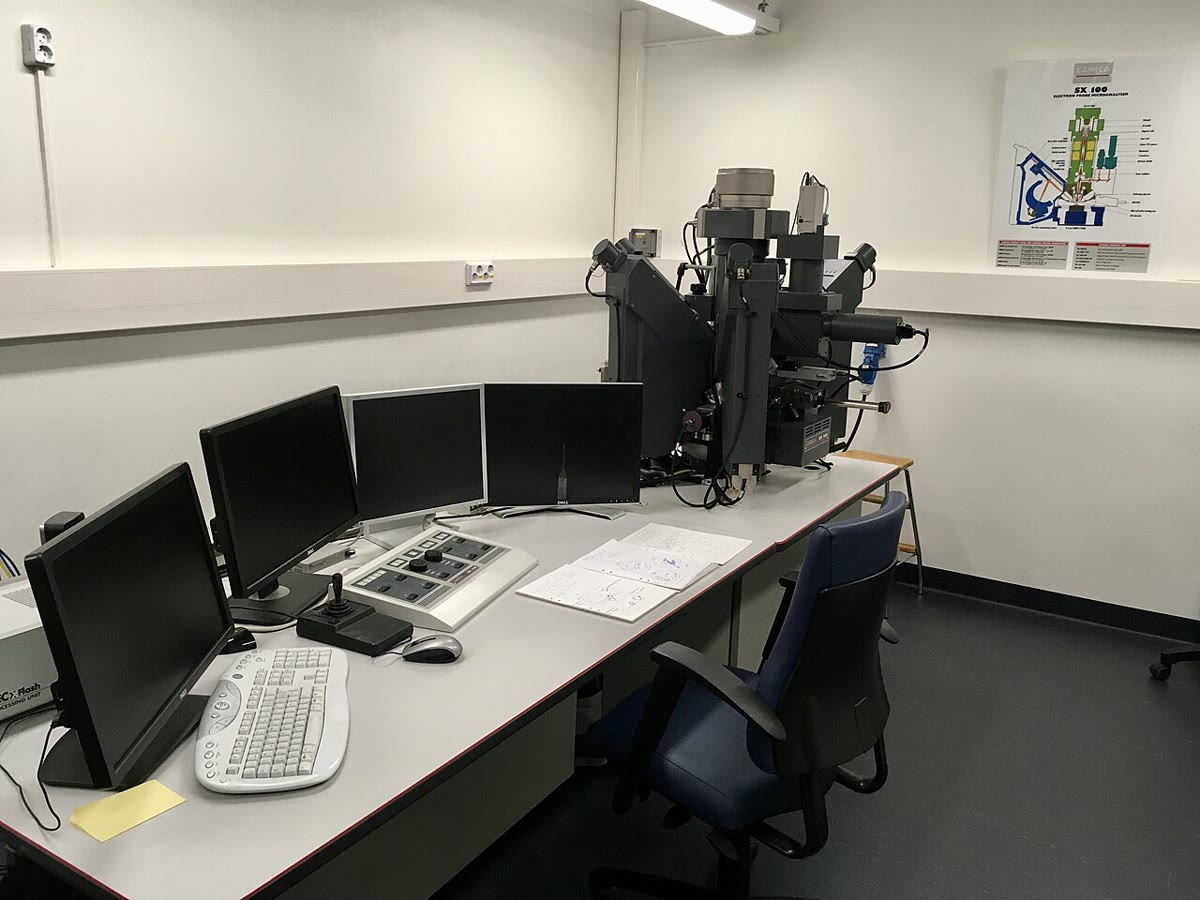
\includegraphics[width=\linewidth]{images/book4/b2-31-microprobe.jpg}
\par\smallskip{\scriptsize Una \omterm{def:b2:field-lab-methods-2:epma}{microsonda electrónica}: la columna electrónica, con sus espectrómetros
alrededor, y la mesa del operador. Fotografía Kallerna, CC BY-SA 4.0 (Wikimedia Commons).}
\end{minipage}
\end{inthelab}
% ledger: sercE:epma-spot, sercE:coating, photo:b2-31-microprobe

\section{Análisis isotópico}\label{sec:b2:field-lab-methods-2:isotopes}

Los \omterm{def:b2:isotope-geochemistry:tracer}{trazadores isotópicos radiogénicos} y las edades (\cref{ch:b2:isotope-geochemistry}) se basan en razones medidas
con una precisión del 0.01--\qty{0.001}{\percent}, sobre elementos separados de la roca por disolución
y cromatografía de intercambio iónico en un laboratorio limpio, con aire filtrado (por lo general de clase 100 a
1000) para que el polvo no añada nada a las pequeñas cantidades analizadas.
% ledger: sercT:tims

\begin{definition}[Espectrometría de masas de ionización térmica, ICP-MS multicolector, sesgo de masa]\label{def:b2:field-lab-methods-2:tims}
En la \emph{espectrometría de masas de ionización térmica}\index{espectrometria de masas de ionizacion termica@espectrometría de masas de ionización térmica} (TIMS, por sus siglas en inglés), un
elemento purificado se deposita sobre una fina cinta metálica y se ioniza calentándolo en vacío; los iones
se aceleran a través de una diferencia de potencial de hasta \qty{10}{kV}, se separan por masa en un sector magnético
y se recogen. En el \emph{ICP-MS multicolector}\index{ICP-MS multicolector} los iones proceden de un
plasma acoplado inductivamente, que ioniza elementos difíciles de ionizar térmicamente, y varios
colectores miden al mismo tiempo los haces de masas distintas. El \emph{sesgo
de masa}\index{sesgo de masa} de una medida es la desviación de una razón isotópica medida respecto de la razón
verdadera de la muestra causada por el instrumento, que transmite o ioniza una masa con más facilidad que
otra.
\end{definition}
% ledger: sercT:tims, sercM:mcicpms

Ambos instrumentos alcanzan esta precisión. La TIMS ioniza en general menos del
\qty{1}{\percent} de los átomos, y su \omterm{def:b2:field-lab-methods-2:tims}{sesgo de masa} cambia continuamente durante una medida. El sesgo se corrige fijando la razón de dos isótopos que ninguna
desintegración modifica, lo que exige un elemento con al menos tres isótopos, dos de ellos estables y no
radiogénicos. Para el estroncio, $^{86}\mathrm{Sr}/^{88}\mathrm{Sr}$ se fija en 0.1194, y una
forma habitual de la corrección es la ley exponencial.
% ledger: sercT:tims, sercM:mcicpms, cheong14:mass-bias, ciaaw:sr-isotopes

\begin{proposition}[Ley exponencial del sesgo de masa]\label{prop:b2:field-lab-methods-2:bias}
Supóngase que toda razón medida de dos isótopos de masas $m_i$ y $m_j$ se relaciona con la razón
verdadera por $R_{ij}^{\mathrm{true}} = R_{ij}^{\mathrm{meas}}\,(m_i/m_j)^{\beta}$, con un único exponente
$\beta$ para toda la medida. Entonces la razón medida $r$ de un par de referencia, cuyo valor verdadero
$r_0$ se conoce, da
\begin{equation}
\beta = \frac{\ln(r_0/r)}{\ln(m_k/m_l)}
\label{eq:b2:field-lab-methods-2:beta}
\end{equation}
para el par de referencia $k/l$, y todas las demás razones se corrigen con el mismo $\beta$.
\end{proposition}

\begin{proof}
Aplicada al par de referencia, la ley se escribe $r_0 = r\,(m_k/m_l)^\beta$; tomando logaritmos,
$\ln(r_0/r) = \beta\ln(m_k/m_l)$, que es \eqref{eq:b2:field-lab-methods-2:beta}. El exponente es
común a todas las razones de la medida por hipótesis, así que corrige cada una de ellas.
\end{proof}

Para el estroncio, el par de referencia es $^{86}\mathrm{Sr}/^{88}\mathrm{Sr}$ con $r_0 = 0.1194$, y
la $^{87}\mathrm{Sr}/^{86}\mathrm{Sr}$ corregida es la razón medida multiplicada por
$(m_{87}/m_{86})^\beta$. Las abundancias de la CIAAW, \qty{9.86}{\percent} de estroncio 86 y
\qty{82.58}{\percent} de estroncio 88, dan el mismo valor. Cada sesión analiza también un \omterm{def:b2:isotope-geochemistry:standards}{patrón isotópico
de referencia}: un laboratorio midió $^{87}\mathrm{Sr}/^{86}\mathrm{Sr} = 0.710252 \pm
0.000007$ en el material de referencia NBS~987 en siete medidas.
% ledger: cheong14:mass-bias, ciaaw:sr-isotopes

Las razones por sí solas no dan una concentración. Para ello, una cantidad conocida de un \emph{trazador enriquecido} (spike), una disolución del
elemento enriquecida artificialmente en un isótopo, se mezcla con la muestra disuelta antes de la
química, y la razón se mide en la mezcla. Los laboratorios de TIMS lo usan tanto para
las concentraciones como para las razones padre--hijo.
% ledger: sercT:tims

\begin{proposition}[Dilución isotópica]\label{prop:b2:field-lab-methods-2:id}
Sean $N_x$ los moles de un isótopo de referencia $b$ en una muestra y $N_s$ los de un trazador enriquecido, y sean
$R_x$, $R_s$ y $R_m$ las razones de un segundo isótopo $a$ a $b$ en la muestra, el trazador y
la mezcla. Entonces
\begin{equation}
N_x = N_s\,\frac{R_s - R_m}{R_m - R_x} .
\label{eq:b2:field-lab-methods-2:id}
\end{equation}
Un error relativo $\varepsilon$ sobre $R_m$ da a $N_x$ el error relativo $\mathcal{M}\varepsilon$,
con el factor de amplificación del error
\begin{equation}
\mathcal{M} = \frac{R_m\,(R_s - R_x)}{(R_s - R_m)(R_m - R_x)} ,
\label{eq:b2:field-lab-methods-2:mag}
\end{equation}
que es mínimo cuando $R_m = \sqrt{R_s R_x}$.
\end{proposition}
\index{dilucion isotopica@dilución isotópica}

\begin{proof}
El isótopo $a$ se conserva en la mezcla: $R_m(N_x + N_s) = R_x N_x + R_s N_s$, así que $N_x(R_m - R_x) =
N_s(R_s - R_m)$, que es \eqref{eq:b2:field-lab-methods-2:id}. Su derivada logarítmica es
$\mathrm{d}\ln N_x/\mathrm{d}\ln R_m = R_m\,[-1/(R_s - R_m) - 1/(R_m - R_x)] = -\mathcal{M}$, con
$\mathcal{M}$ como en \eqref{eq:b2:field-lab-methods-2:mag}. Salvo la constante positiva $R_s - R_x$,
$1/\mathcal{M} = (R_s - R_m)(R_m - R_x)/R_m = R_s + R_x - R_m - R_sR_x/R_m$, cuya derivada
$-1 + R_sR_x/R_m^2$ se anula en $R_m = \sqrt{R_sR_x}$, un máximo de $1/\mathcal{M}$.
\end{proof}

La \omterm{prop:b2:field-lab-methods-2:id}{dilución isotópica} no necesita ni una recta de calibración ni una recuperación completa del elemento a lo largo de
la química: una vez mezclados trazador y muestra, las pérdidas afectan a ambos por igual. Un trazador de estroncio
publicado, por ejemplo, contiene un \qty{99.65}{\percent} de estroncio 84, con
$^{84}\mathrm{Sr}/^{88}\mathrm{Sr} = 561.4$ y $^{86}\mathrm{Sr}/^{88}\mathrm{Sr} = 0.7661$, a razón de
\qty{15.271}{\micro\gram} de estroncio por gramo de disolución. Su razón 86/88 muestra por qué el \omterm{def:b2:field-lab-methods-2:tims}{sesgo
de masa} de una mezcla con trazador no puede corregirse fijando $^{86}\mathrm{Sr}/^{88}\mathrm{Sr}$ en su
valor natural: el trazador ha desplazado esa razón.
% ledger: cheong14:spike, cheong14:mass-bias

\section{Una campaña de cartografía en el asomo de Varden}\label{sec:b2:field-lab-methods-2:campaign}

En el núcleo del anticlinal de Varden, la erosión ha atravesado la cobertera de arenisca y ha dejado al descubierto el
basamento: esquisto intruido por un granito. Una campaña destinada a abastecer al laboratorio empieza en el
campo. Se recorren dos itinerarios de oeste a este a través del asomo, con una estación cada
\qty{100}{m}; en cada una se anota la unidad, y se toman muestras frescas donde la roca no está
meteorizada, numeradas con la estación y, donde hay que medir fábricas, orientadas. La figura
muestra lo que encuentran las estaciones: de las 30, diez están sobre granito, diez sobre la cobertera de arenisca, una sobre
el esquisto, una sobre caliza y ocho sobre el aluvión del fondo del valle, donde no aflora
ninguna roca.

\begin{omfigure}
\centering
\begin{tikzpicture}
\begin{axis}[axis equal image, xmin=2.4, xmax=4.6, ymin=3.1, ymax=5.0, width=0.66\linewidth,
  tick label style={font=\scriptsize}, xlabel={este (km)}, ylabel={norte (km)},
  label style={font=\small}]
% units: figdata/shared/region.py (read only); stations: figdata/bachelor-2/labmethods.py part stations
\addplot[lith schist, draw=black, line width=0.3pt, even odd rule] table {figdata/out/shared-region-unit-schist.dat};
\addplot[lith granite, draw=black, line width=0.3pt, even odd rule] table {figdata/out/shared-region-unit-granite.dat};
\addplot[om lith={icsTriassic!35}{om sand}, draw=black, line width=0.3pt, even odd rule] table {figdata/out/shared-region-unit-sandstone.dat};
\addplot[om lith={icsJurassic!40}{om limestone}, draw=black, line width=0.3pt, even odd rule] table {figdata/out/shared-region-unit-limestone.dat};
\addplot[om lith={icsJurassic!15}{om shale}, draw=black, line width=0.3pt, even odd rule] table {figdata/out/shared-region-unit-shale.dat};
\addplot[lith alluvium, draw=black, line width=0.3pt, even odd rule] table {figdata/out/shared-region-unit-alluvium.dat};
\addplot[river] table {figdata/out/shared-region-river.dat};
\addplot[only marks, mark=*, mark size=1.6pt, mark options={fill=white, draw=black}]
  table[x=x_km, y=y_km] {figdata/out/bachelor-2-labmethods-stations.dat};
\addplot[only marks, mark=*, mark size=1.6pt, mark options={fill=omThm, draw=black},
  x filter/.expression={\thisrow{unit}==2 ? x : nan}]
  table[x=x_km, y=y_km] {figdata/out/bachelor-2-labmethods-stations.dat};
\node[font=\scriptsize, fill=white, inner sep=1pt, anchor=east] at (axis cs:2.76,3.7) {1};
\node[font=\scriptsize, fill=white, inner sep=1pt, anchor=west] at (axis cs:4.24,3.7) {15};
\node[font=\scriptsize, fill=white, inner sep=1pt, anchor=east] at (axis cs:2.76,4.4) {16};
\node[font=\scriptsize, fill=white, inner sep=1pt, anchor=west] at (axis cs:4.24,4.4) {30};
\draw[black, line width=0.5pt] (axis cs:3.5,4.44) -- (axis cs:3.5,4.62);
\node[font=\scriptsize, fill=white, inner sep=1pt, anchor=south] at (axis cs:3.5,4.62) {estación 23};
\pic at (axis cs:4.45,4.75) {northarrow};
\end{axis}
\end{tikzpicture}
\par\smallskip{\small El asomo del basamento de las colinas de Varden con las 30 estaciones de dos itinerarios
oeste--este, separados \qty{100}{m}. Puntos rojos: estaciones sobre granito. Rosa con cruces: granito; gris: esquisto; morado: arenisca
triásica; azul: caliza jurásica; azul claro: lutita jurásica; crema: aluvión del río, que
fluye hacia el este. La
muestra de granito del problema de fin de semana procede de la estación 23.}
\end{omfigure}

\begin{inthefield}[Muestreo para el laboratorio]
\centering
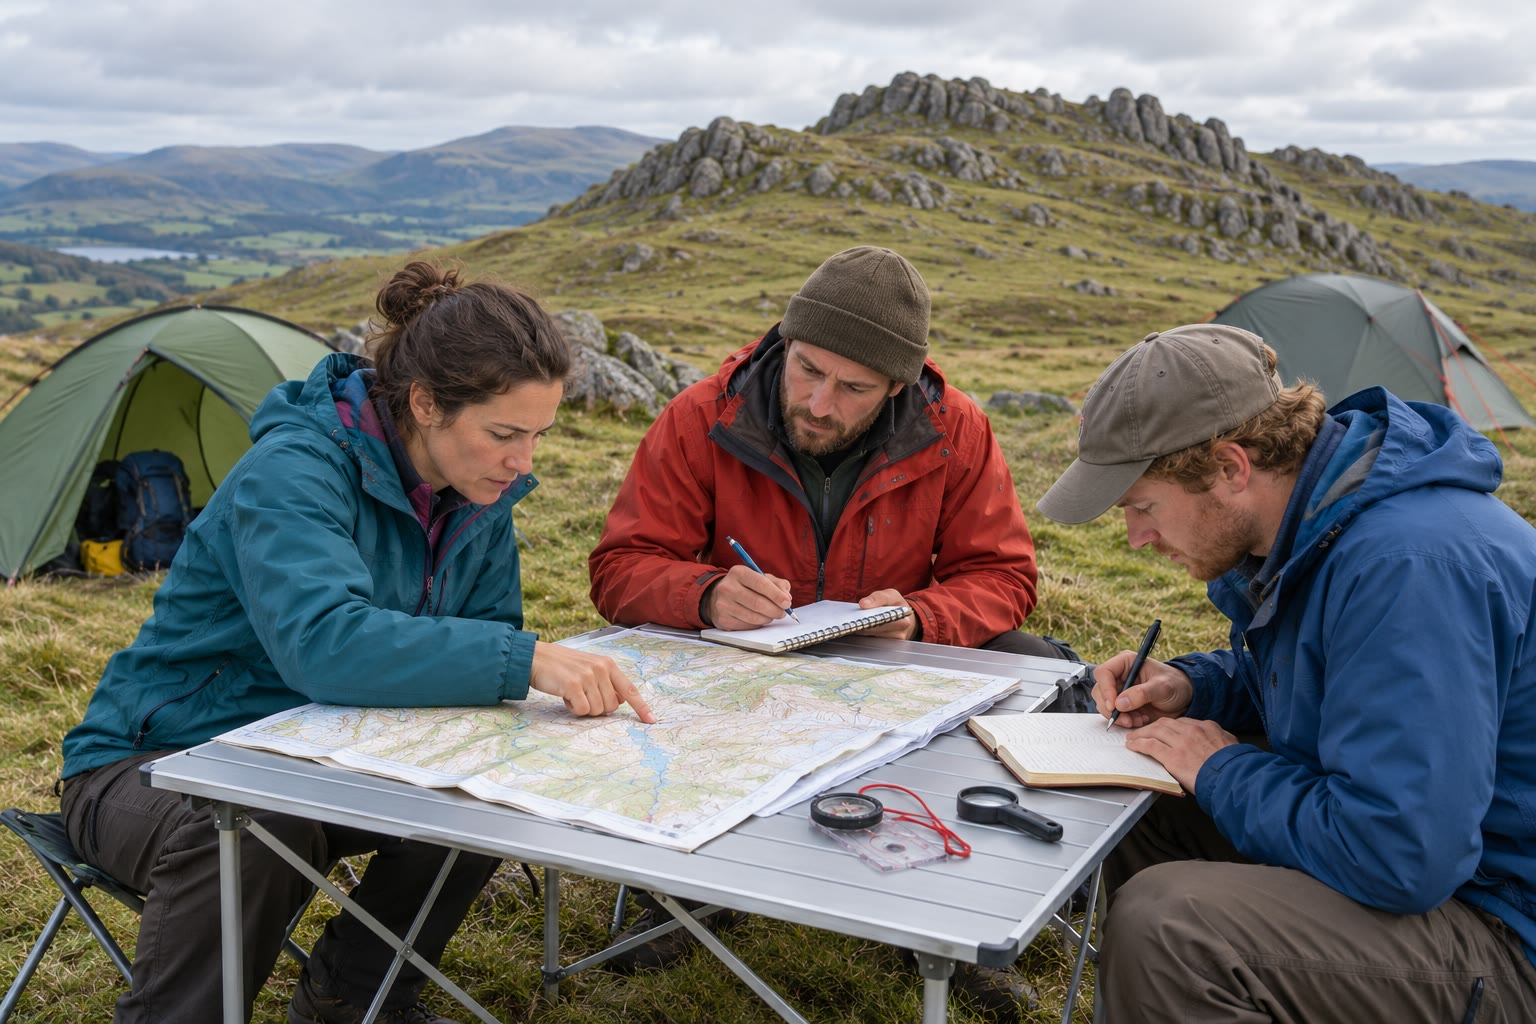
\includegraphics[width=0.56\linewidth]{images/book4/ai/b2-field-camp.jpg}
\par\smallskip{\small Un equipo de campo planifica los itinerarios del día siguiente (ilustración generada por IA).}
\par\medskip\raggedright
Por la tarde, el equipo traslada las estaciones al mapa, comprueba que cada número de muestra de los
cuadernos corresponde a una bolsa y decide qué muestras van a qué laboratorio. Una muestra de cada unidad
va al laboratorio de láminas delgadas; el granito y el esquisto más frescos van
a trituración y análisis de roca total; unas pocas muestras de granito se reservan para los isótopos. El
número de estación acompaña a cada muestra en cada paso, de la bolsa a la lámina delgada, el
polvo, la perla y la línea de una tabla de datos, de modo que cualquier resultado extraño pueda rastrearse hasta su
afloramiento.
\end{inthefield}

\section{La calidad de un número}\label{sec:b2:field-lab-methods-2:quality}

Cada paso de la cadena añade su propio error, y los métodos de este capítulo muestran los dos tipos que
distinguen los libros de química. El \omterm{def:b2:field-lab-methods-2:modal}{recuento de puntos} y las razones isotópicas tienen sobre todo errores aleatorios, que
disminuyen a medida que crecen los recuentos, como $1/\sqrt n$; la calibración tiene errores sistemáticos, que la repetición no
reduce y que solo revela un material de referencia. La figura de los análisis de sílice muestra
ambos: las barras son la precisión del método, y un punto que se aparta de cero en muchas veces su barra
dividida por la raíz cuadrada del número de análisis indica un sesgo. El mismo elemento medido por dos
métodos, el estroncio por XRF y por \omterm{prop:b2:field-lab-methods-2:id}{dilución isotópica}, es un control adicional, ya que los dos no comparten ninguna
calibración. Los resultados se dan con su incertidumbre, redondeados de acuerdo con ella, y con los materiales de
referencia analizados junto a ellos; un número sin ellos no puede compararse con ningún otro.

\section*{Ejercicios}\label{sec:b2:field-lab-methods-2:exercises}

Datos de los ejercicios, salvo aviso contrario: masas atómicas H 1.008, O 15.999, Mg 24.305, Al
26.982, Si 28.085, K 39.098, Sr 87.62; masas isotópicas $^{86}\mathrm{Sr}$ 85.909261,
$^{87}\mathrm{Sr}$ 86.908878, $^{88}\mathrm{Sr}$ 87.905612; estroncio natural,
$^{84}\mathrm{Sr}/^{86}\mathrm{Sr} = 0.05680$, \qty{9.86}{\percent} de $^{86}\mathrm{Sr}$; el trazador
del texto, $^{84}\mathrm{Sr}/^{86}\mathrm{Sr} = 732.8$, \qty{0.13599}{\percent} de
$^{86}\mathrm{Sr}$, peso atómico 83.9242, \qty{15.271}{\micro\gram\per\gram}. Redondéese a tres
cifras significativas salvo indicación contraria.
% ledger: ciaaw:H, ciaaw:O, ciaaw:Mg, ciaaw:Al, ciaaw:Si, ciaaw:K, ciaaw:sr-isotopes, cheong14:spike

\begin{exercise}[$\star$]\label{exo:b2:field-lab-methods-2:1}
(a) Nómbrese la textura o el cristal: (i) una dolerita en la que listones de plagioclasa están totalmente englobados en
grandes cristales de augita; (ii) un mármol de granos de calcita de igual tamaño cuyos límites rectos se encuentran de
tres en tres; (iii) un cristal de estaurolita de \qty{5}{mm} de largo repleto de inclusiones de cuarzo en un esquisto micáceo;
(iv) un granate rodeado por un borde continuo de plagioclasa y piroxeno. (b) Tres límites de grano
se encuentran formando ángulos de \ang{104}, \ang{128} y \ang{128}. Hállese la razón entre la tensión del límite opuesto
al ángulo de \ang{104} y la de los otros.
\end{exercise}

\begin{exercise}[$\star$]\label{exo:b2:field-lab-methods-2:2}
Una roca de grano grueso contiene un \qty{25}{\percent} de cuarzo, 15 de feldespato alcalino, 40 de plagioclasa, 12 de
biotita y 8 de hornblenda. (a) Recalcúlense Q, A y P. (b) Hállese P/(A+P) y nómbrese la roca. (c) Hállese
su índice de color y califíquese.
\end{exercise}

\begin{exercise}[$\star$]\label{exo:b2:field-lab-methods-2:3}
Un recuento de 800 puntos encuentra un mineral al \qty{12}{\percent}. (a) Hállese la desviación típica de
esta proporción, y su valor relativo. (b) ¿Cuál sería con 3200 puntos?
\end{exercise}

\begin{exercise}[$\star$]\label{exo:b2:field-lab-methods-2:4}
Un polvo de \qty{0.8000}{g} pesa \qty{0.7712}{g} tras la calcinación, y el residuo se funde con
\qty{8.0000}{g} de fundente. (a) Hállese la \omterm{def:b2:field-lab-methods-2:xrf}{pérdida por calcinación}. (b) Hállese la fracción másica de la muestra en
la perla. (c) El vidrio contiene un \qty{5.20}{\percent} de \ce{SiO2}. Hállese la sílice del polvo calcinado
y la del polvo original.
\end{exercise}

\begin{exercise}[$\star\star$]\label{exo:b2:field-lab-methods-2:5}
(a) ¿Cuántos puntos se necesitan para medir un mineral accesorio que constituye el \qty{2}{\percent} de una roca
con un error típico relativo del \qty{10}{\percent}? (b) ¿Y un mineral que constituye el \qty{30}{\percent},
con el mismo error relativo? (c) Coméntese el esfuerzo que exige un mineral escaso.
\end{exercise}

\begin{exercise}[$\star\star$]\label{exo:b2:field-lab-methods-2:6}
En los resultados del USGS de la figura, la riolita RGM-1 dio \ce{SiO2} $= 72.89$ con una desviación
típica de 0.19 en 20 análisis (recomendado 73.45), y el basalto BCR-2 dio 54.17 con 0.13 en
20 análisis (recomendado 54.1). (a) Hállese la recuperación de cada uno, en tanto por ciento. (b) Hállese la desviación
típica de cada media, y exprésese cada diferencia respecto del valor recomendado en unidades de ella.
(c) ¿Qué resultado muestra un sesgo? ¿Es el método menos preciso para RGM-1?
\end{exercise}

\begin{exercise}[$\star\star$]\label{exo:b2:field-lab-methods-2:7}
Se quiere comprobar un análisis de microsonda de una flogopita pura, $\mathrm{KMg_3AlSi_3O_{10}(OH)_2}$.
(a) Hállense la masa molar de la fórmula y la fracción másica de \ce{H2O} que contiene. (b) Hállense las
fracciones másicas de \ce{K2O}, \ce{MgO}, \ce{Al2O3} y \ce{SiO2}, y el total que daría un análisis
exacto. (c) ¿Por qué un total de alrededor del \qty{96}{\percent} para una mica no es un mal análisis?
\end{exercise}

\begin{exercise}[$\star\star$]\label{exo:b2:field-lab-methods-2:8}
Una medida de TIMS sobre un patrón de estroncio da $^{86}\mathrm{Sr}/^{88}\mathrm{Sr} = 0.11905$ y
$^{87}\mathrm{Sr}/^{86}\mathrm{Sr} = 0.71062$. (a) Hállese el exponente $\beta$ de la ley exponencial.
(b) Corríjase la razón $^{87}\mathrm{Sr}/^{86}\mathrm{Sr}$, con cinco decimales. (c) ¿Se vio favorecido en la medida el isótopo
ligero o el pesado?
\end{exercise}

\begin{exercise}[$\star\star$]\label{exo:b2:field-lab-methods-2:9}
Para controlar su \omterm{prop:b2:field-lab-methods-2:id}{dilución isotópica}, un laboratorio añade a \qty{0.0500}{g} del basalto de referencia BHVO-2
\qty{0.1000}{g} del trazador del texto, y mide $^{84}\mathrm{Sr}/^{86}\mathrm{Sr} =
0.874$ en la mezcla. (a) Hállense los moles de $^{86}\mathrm{Sr}$ en la alícuota de trazador. (b) Hállense los
moles de $^{86}\mathrm{Sr}$ en la muestra, y su concentración de estroncio en ppm. (c) Compárese con
los \qty{394.1}{ppm} recomendados.
\end{exercise}

\begin{exercise}[$\star\star\star$]\label{exo:b2:field-lab-methods-2:10}
Para el trazador de estroncio del texto ($R_s = 732.8$, $R_x = 0.05680$): (a) hállese la razón de mezcla
que minimiza el factor de amplificación del error, y su valor en ese punto; (b) evalúese $\mathcal M$ para
$R_m = 0.1$, 0.5, 1.664 y 100; (c) explíquese por qué debe evitarse una mezcla próxima a cualquiera de los dos miembros
extremos, y cuánta libertad tiene en la práctica el analista.
\end{exercise}

\begin{exercise}[$\star\star\star$]\label{exo:b2:field-lab-methods-2:11}
Un recuento en un granito encuentra 400 puntos de feldespato, el \qty{62}{\percent} de ellos de plagioclasa. (a) Tratando la
plagioclasa entre los puntos de feldespato como un recuento binomial, hállese la desviación típica de
P/(A+P). (b) ¿A cuántas desviaciones típicas está el resultado del límite con la granodiorita? (c) ¿Cuántos
puntos de feldespato lo situarían a dos desviaciones típicas del límite?
\end{exercise}

\begin{exercise}[$\star\star\star$]\label{exo:b2:field-lab-methods-2:12}
Un mineral ocupa una fracción $p$ de una roca. (a) Demuéstrese que la probabilidad de que $n$ puntos independientes
fallen todos es $(1-p)^n$. (b) ¿Cuántos puntos dan al menos un \qty{95}{\percent} de probabilidad de
acertar al menos una vez un mineral que constituye el \qty{1}{\percent} de la roca? (c) Lo mismo para el circón al
\qty{0.05}{\percent}, y conclúyase cómo debe buscarse un mineral accesorio.
\end{exercise}

\section*{Problema de fin de semana}

\begin{problem}[{Problema de fin de semana --- Del afloramiento al análisis}]\label{pb:b2:field-lab-methods-2:1}
% invented sample; data: ledger rows below; values: calc/ch31.py
La muestra VH-23 del granito de Varden se tomó en la estación 23 de la campaña. En una lámina delgada se hizo un
\omterm{def:b2:field-lab-methods-2:modal}{recuento de puntos} sobre una malla regular de 1200 puntos: cuarzo 372, feldespato alcalino 348, plagioclasa 324,
biotita 108, moscovita 36, óxidos opacos 12. Un polvo de \qty{0.8000}{g} pesó \qty{0.7949}{g}
tras la calcinación a \qty{925}{\celsius} y se fundió con \qty{8.0000}{g} de fundente. Perlas de tres
materiales de referencia dieron estas intensidades de \ce{SiO2} (miles de cuentas por segundo, kcps): BCR-2,
recomendado \qty{54.1}{\percent}, 21.66; AGV-2, 59.3, 23.70; RGM-1, 73.45, 29.37; la perla de granito
dio 28.63. Los demás óxidos del granito suman un \qty{27.15}{\percent}. Para los isótopos,
se disolvieron \qty{0.1000}{g} de polvo y se mezclaron con \qty{0.2500}{g} del trazador del texto;
se supone que la muestra tiene las abundancias naturales de estroncio de los ejercicios. Úsense los datos de los
ejercicios.

\noindent\textbf{Parte I --- La moda.}
\begin{enumerate}
  \item Hállese la proporción modal de cada mineral.
  \item Hállense la desviación típica de la proporción de cuarzo y la desviación típica relativa
        de la proporción de moscovita.
  \item Hállense $M$ y el índice de color $M'$, y califíquese la roca.
  \item Recalcúlense Q, A y P a una suma de 100.
  \item Hállese P/(A+P) y nómbrese la roca en el \omterm{def:b2:magmatic-series:qapf}{diagrama QAPF}.
  \item Con la desviación típica binomial de P/(A+P) sobre los 672 puntos de feldespato, ¿es seguro
        el nombre?
  \item ¿Cuántos puntos llevarían la desviación típica de la proporción de cuarzo a un punto
        porcentual?
\end{enumerate}

\noindent\textbf{Parte II --- La sílice por fluorescencia de rayos X.}
\begin{enumerate}[resume]
  \item Hállese la \omterm{def:b2:field-lab-methods-2:xrf}{pérdida por calcinación}.
  \item Hállense la fracción másica de la muestra en la perla y la sílice del vidrio si el
        polvo calcinado contiene un \qty{72}{\percent}.
  \item Ajústese la recta de mínimos cuadrados $c = aI + b$ por los tres materiales de referencia; dense $a$ con
        cuatro decimales y $b$ con dos.
  \item Hállese el \ce{SiO2} del granito, con dos decimales.
  \item Hállense los residuos de los tres materiales de referencia. ¿Es adecuada la recta?
  \item Súmense los óxidos y la \omterm{def:b2:field-lab-methods-2:xrf}{pérdida por calcinación}. ¿Repetiría este análisis el procedimiento del USGS?
  \item Recalcúlese la sílice a una suma de 100 sin los volátiles.
\end{enumerate}

\noindent\textbf{Parte III --- El sesgo de masa.}
\begin{enumerate}[resume]
  \item A partir de las abundancias de la CIAAW, hállese la $^{86}\mathrm{Sr}/^{88}\mathrm{Sr}$ natural y compárese
        con el valor usado para normalizar.
  \item Una alícuota sin trazador da $^{86}\mathrm{Sr}/^{88}\mathrm{Sr} = 0.11853$. Hállese $\beta$ con
        cuatro decimales.
  \item Da $^{87}\mathrm{Sr}/^{86}\mathrm{Sr} = 0.71655$. Corríjase, con cinco decimales.
  \item Hállese el sesgo por unidad de masa, en tanto por ciento.
  \item ¿Por qué no puede hacerse esta corrección sobre la mezcla con trazador de la parte IV?
\end{enumerate}

\noindent\textbf{Parte IV --- Dilución isotópica.}
\begin{enumerate}[resume]
  \item Compruébese que el trazador contiene un \qty{99.65}{\percent} de estroncio 84 y un \qty{0.13599}{\percent}
        de estroncio 86.
  \item Hállense los moles de estroncio y de $^{86}\mathrm{Sr}$ en la alícuota de trazador, con cuatro
        cifras significativas.
  \item Compruébense los valores $R_s = 732.8$ y $R_x = 0.05680$ de los ejercicios.
  \item La razón corregida de la mezcla es $R_m = 1.6812$. Hállense los moles de $^{86}\mathrm{Sr}$
        de la muestra.
  \item Hállese el factor de amplificación del error. Con $R_m$ conocida al \qty{0.01}{\percent} y la concentración del
        trazador a $\pm\qty{0.031}{\micro\gram\per\gram}$, hállese la incertidumbre relativa
        del resultado.
  \item Hállese la concentración de estroncio del granito de Varden, en ppm.
\end{enumerate}
\end{problem}
% ledger: bgsI:qapf, bgsI:colour-index, usgsT:procedure, usgsT:sio2-table, ciaaw:sr-isotopes, cheong14:spike, cheong14:mass-bias
